\section{Results} % (fold)
\label{sec:results}

 

\subsection{LDA} % (fold)
\label{sub:lda}

The results from the LDA depends on the amount of topics specified. This requires consideration on two parts: First is whether the amount of topics specified makes intuitive sense. The second is what amount of topics produces the highest gift prediction accuracy. Therefore, I created an infrastructure to model a wide set of topics ranging from 2 to 10, and thereafter different intervals ranging from 10 up till a 100 topics\footnote{the source files provided for this paper shows all of the topics modeled as well as figures representing all of the topics. Each of the figures presented in this paper has counterparts for all of the topics in the sources files.}. These  are useful for computing different regression and neural network predictions. However, I stick with 30 topics for the purpose of this section to show how the model performed\footnote{Although there exist test to check the optimal amount of topics within a dataset (such as those developed by \cite{arun2010finding}, \cite{griffiths2004finding} and more) the amount of topics used in this section is based on intuition and is meant to represent the results from the modeling.}. 

\

Figure 3 below represents the product distributions over each of the 30 topics. In other words, the figure shows the total documents likely to be within each topic; each product's, or document's, maximum gamma probability value is taken, thereby allocating it to only a specific topic, thereafter each topic is counted for the amount of products within each topic. The figure shows a good distribution of products over the topics, meaning that the topics do capture a variety of products. This is the aim of using the Wikipedia descriptions of the products, to allocate them into distinct topics without having a single topic, or a set of topics, dominate the entire product space. 


\begin{figure}[!h]
\caption{Product-Topic Distribution}\centering
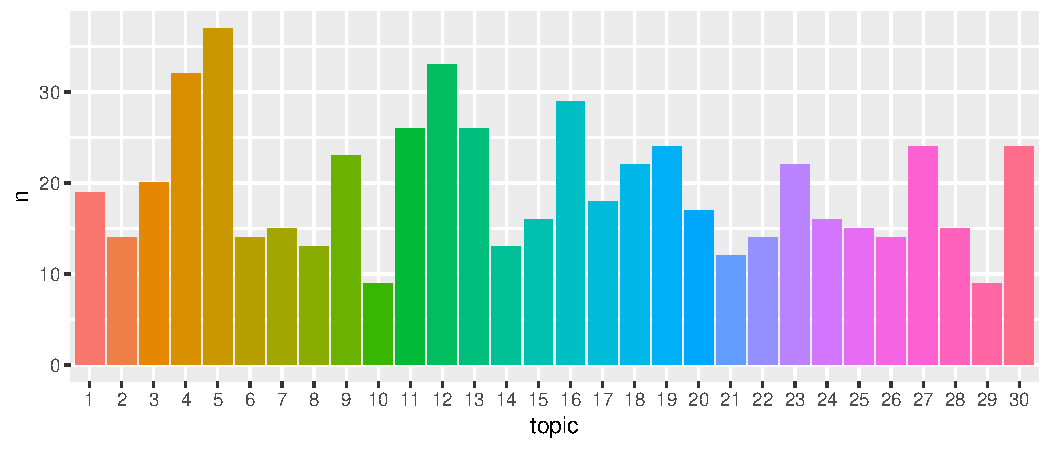
\includegraphics[width=0.9\textwidth]{/Users/charlvanschoor/Documents/Gottingen/ML/ML-Applications-CVS/LDA_consumer_analysis/src/output/product-distribution-per-topic/product-distribution-per-30-topic.pdf}
\end{figure}


\begin{figure}[!h]
\caption{Product-Topic Mixture}\centering
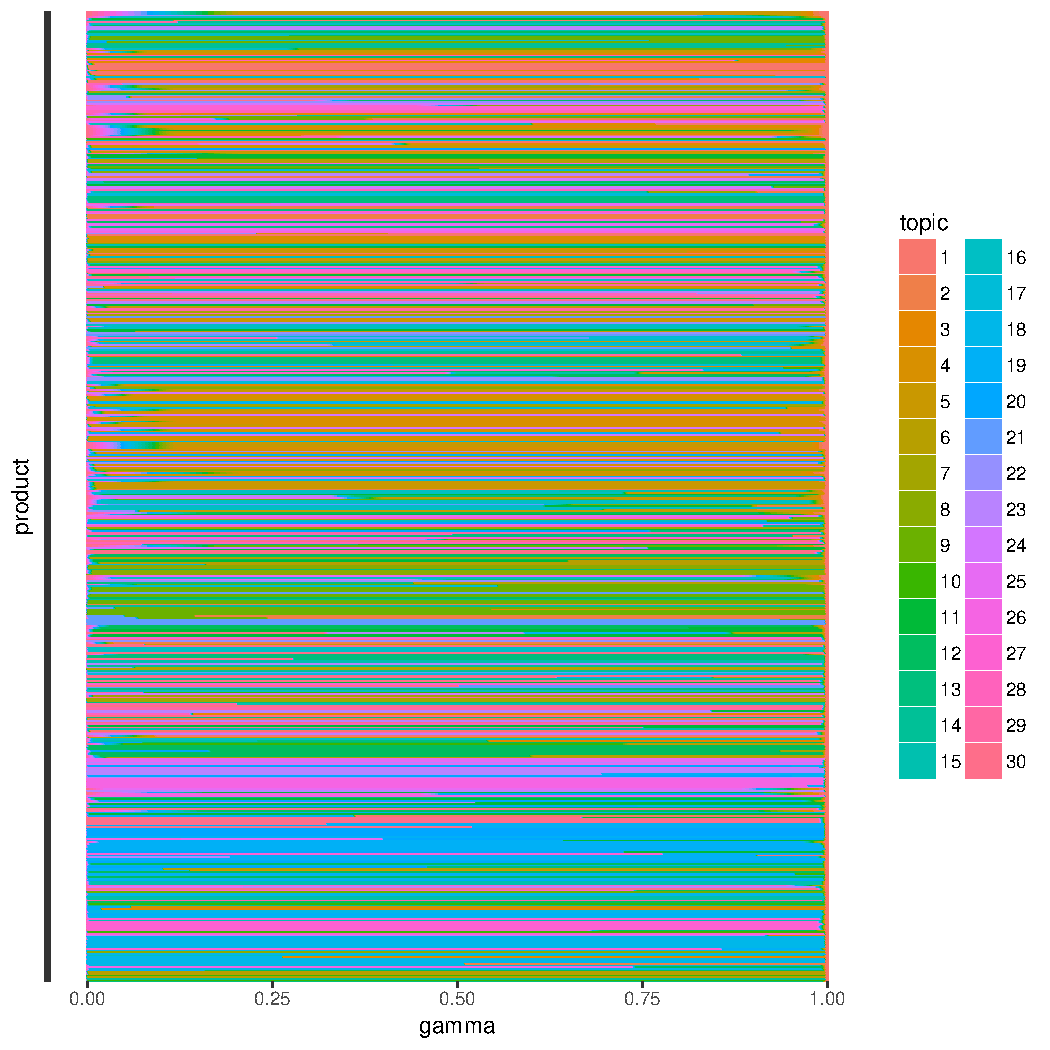
\includegraphics[width=0.9\textwidth]{/Users/charlvanschoor/Documents/Gottingen/ML/ML-Applications-CVS/LDA_consumer_analysis/src/output/topic-distributions-per-product/30-topic-distribution-per-product.pdf}
\end{figure}
\

Moreover, Figure 4 shows a similar story as that of the one above; it shows the gamma probability distributions for each of the products, or documents. In other words, the figure shows the probabilities for each document belonging to each of the 30 topic\footnote{The sources files provided for this paper contains figures representing this for all of the topic sets.}. As visible from the figure, most products are allocated to specific topics; this indicates that most products fall within a certain topic, which is a good result given the origin of the text data. However, some products belong to various topics. Once again, this is not a bad result as it gives some variance to the model. This means that the LDA possibly allocated a probability for complimentary products into the same topics, and probabilities for substitute products into other topics. In other words, some products belong to each other, like vehicles and fuel, and the LDA allocated higher probabilities to those products in the same topic. Some products are substitutes products, like sugar and artificial sweeteners for example, and the LDA possibbly allocated probabilities for those products in the same topic. This means that the LDA might be picking up relationships between the products that are not available when considering the products on their own; it would be tedious for a person to allocate more than 500 products into topics. 


\

\begin{figure}[!h]
\caption{Top 6 Words Over 30 Topics}\centering
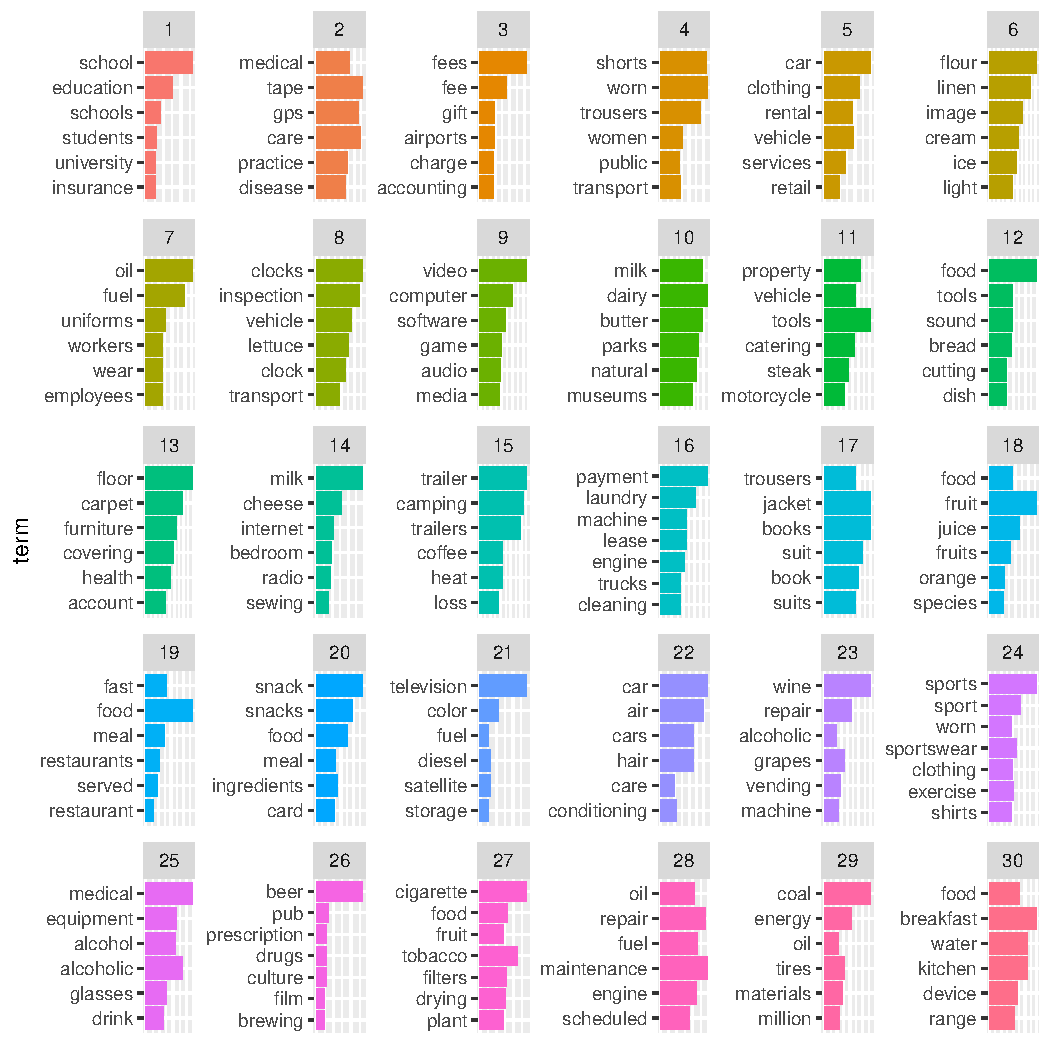
\includegraphics[width=0.9\textwidth]{/Users/charlvanschoor/Documents/Gottingen/ML/ML-Applications-CVS/LDA_consumer_analysis/src/output/top-words-per-topic/top-6-words-in-each30-topics.pdf}
\end{figure}

Figure 5 emphasizes the point made above. The figure shows top 6 words (the maximum beta probabilities for each word) in the 30 topics. There are a few notable topics: Topic 1 represents electronic devices, topic 2 consists of food products, topic 7 represents camping related products and services, topic 12 consists of fast food and restaurant products, topic 23 represents clothing items, topic 29 connects cultural activities etc. The figure shows that the model was able to allocate products that are related to each other. This emphasizes the point that a LDA model requires more information in the documents to allocate products into topics. The result is a mixture of product in each topic that are related in some way, by either cultural or economic principles\footnote{As an economic example, topic 21 relates education with public transport, which makes sense as students use public transport.}. 




% subsection lda (end)


\subsection{Logistic Regression} % (fold)
\label{sub:logistic_regression}


The results from the logistic regression show a compelling story for the inclusion of topics into the model. However, the models seems to show endogeneity, as the significance of the topics far outstretch the significance of the control variables. This is due to the prediction variable used for the model; it is intuitive that the relationship between product and gift purchases is strong, as the one is a direct result of the other. I controlled for this, to some extent, by allocating a binary value to whether a consumer purchased a gift or not, as this eliminates some of the direct relationship between the values. The results do however tell a story, thus we proceed. 

\

Figure 6 shows the top 20 coefficients in terms of significance (sorted by p-value) for the logistic regression that included a 100 topics. The reasoning behind using 100 topics as a representation of the model is due to a few statistics indicating the accuracy and the explanatory power of the model\footnote{The source files provided for this paper contains the results for all of the models with a different set of topics.}. The top 20 predictors are sorted from lowest to the highest p-value. It is clear from the figure that the most significant predictors are the topics\footnote{The source files show that with less topics, around 40, more of the demographic variables are of importance; an intuitive result.}. Topic 73 is the most significant in explaining and predicting gift purchasing behaviour, where topic 99 is the 20th most significant predictor. It is interesting, and intuitive, to note that AGE is the 7th most significant predictor, indicating that generally older households tend to purchase more gifts. The top predictor topics, after inspecting the dataset, contained words such as vehicle, property, truck, agreement, school, bus, students, united, shorts, trousers, sports, electronic etc. Interpreting these results is however difficult, as one does not know exactly what the relationships the topics capture. 

\begin{figure}[!h]
\caption{Top 20 Predictors for 100 Topics}\centering
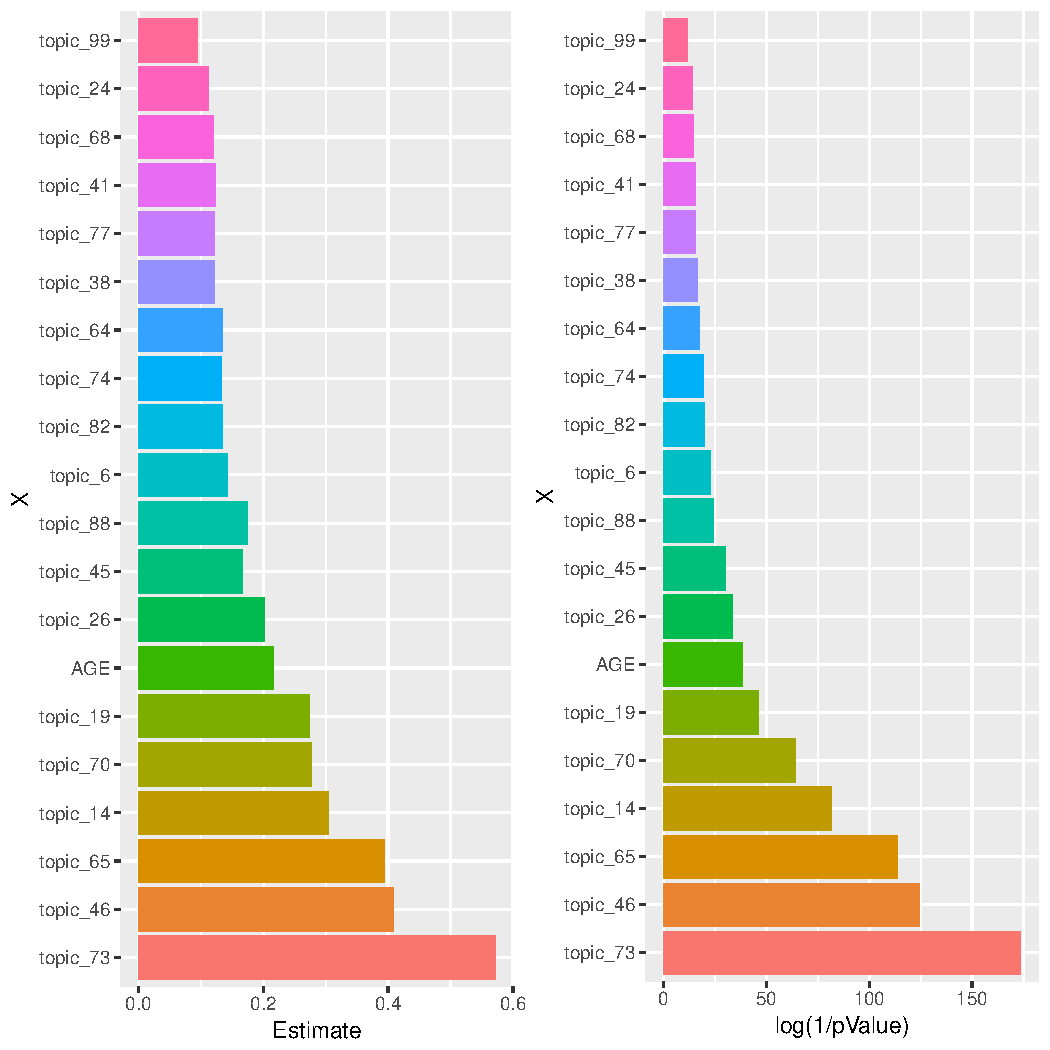
\includegraphics[width=0.7\textwidth]{/Users/charlvanschoor/Documents/Gottingen/ML/ML-Applications-CVS/LDA_consumer_analysis/src/output/GLM-significantPlots/sigPvalue_NUM_TOPICS100.pdf}
\end{figure}

\

It is clear thought that purchases of these types of products are strongly related to gift purchasing behaviour. Note that all of the top predictors are positive, meaning that all increase the likelihood of gift purchasing behaviour. One can speculate that households with property, vehicles, social agreements, children as students etc. have a higher probability of buying gifts. This follows on the intuition of the theoretical background of this paper: Individuals that consider the outcome of their purchases are more probable to exhibit gift giving behaviour. 

\

Figures 7 and 8 show the predictive capability of the logistic regression model. Figure 7 is the confusion matrix from using the 100 topics. As visible from the graph, the model is able to predict non-gift purchasing behaviour well, 86 percent accuracy, but not well with predicting gift purchasing behaviour, 55 percent accuracy. 

\

Moreover, Figure 8 shows various statistics for the model. Some important elements are the Mcfadden R-square value and the balanced accuracy. The Mcfadden R-square value is only 25 percent, meaning that the model as a whole has low explanatory power\footnote{The R-square value for the models with less topics are less than the R-square value for the 100 topic model.}. Moreover, the balanced accuracy, which is a measurement for the predictive power, is 70 percent. In other words, the model only predicts false positives and false negatives 30 percent of the time. Thus, the model does have some predictive capability, but lacks in the prediction of gift purchasing behaviour. 


\begin{figure}[!h]
\caption{Confusion Matrix: Top 20 Predictors for 100 Topics}\centering
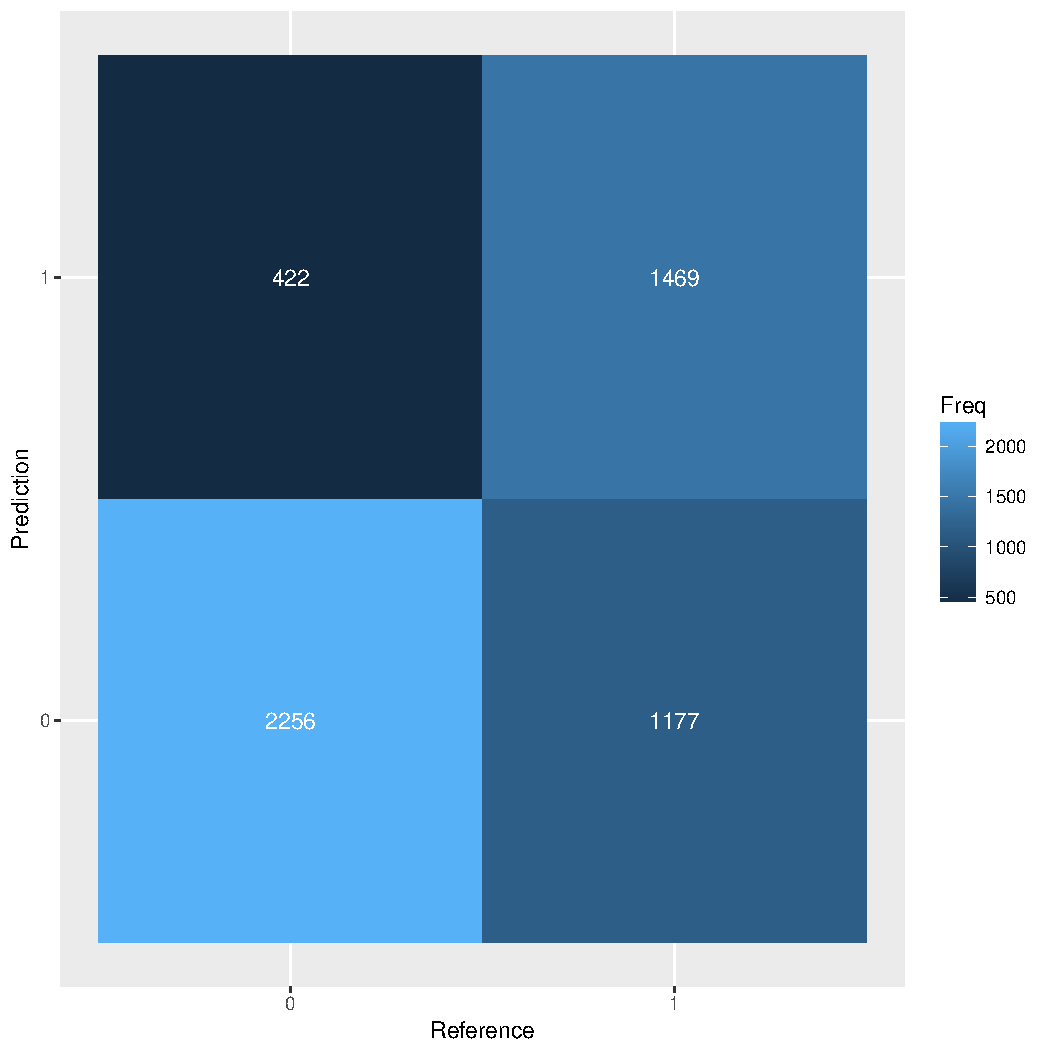
\includegraphics[width=0.5\textwidth]{/Users/charlvanschoor/Documents/Gottingen/ML/ML-Applications-CVS/LDA_consumer_analysis/src/output/confusion-matrices/conf-matrix_NUM_TOPICS100.pdf}
\end{figure}

\begin{figure}[!h]
\caption{Auxiliary Statistics: Top 20 Predictors for 100 Topics}\centering
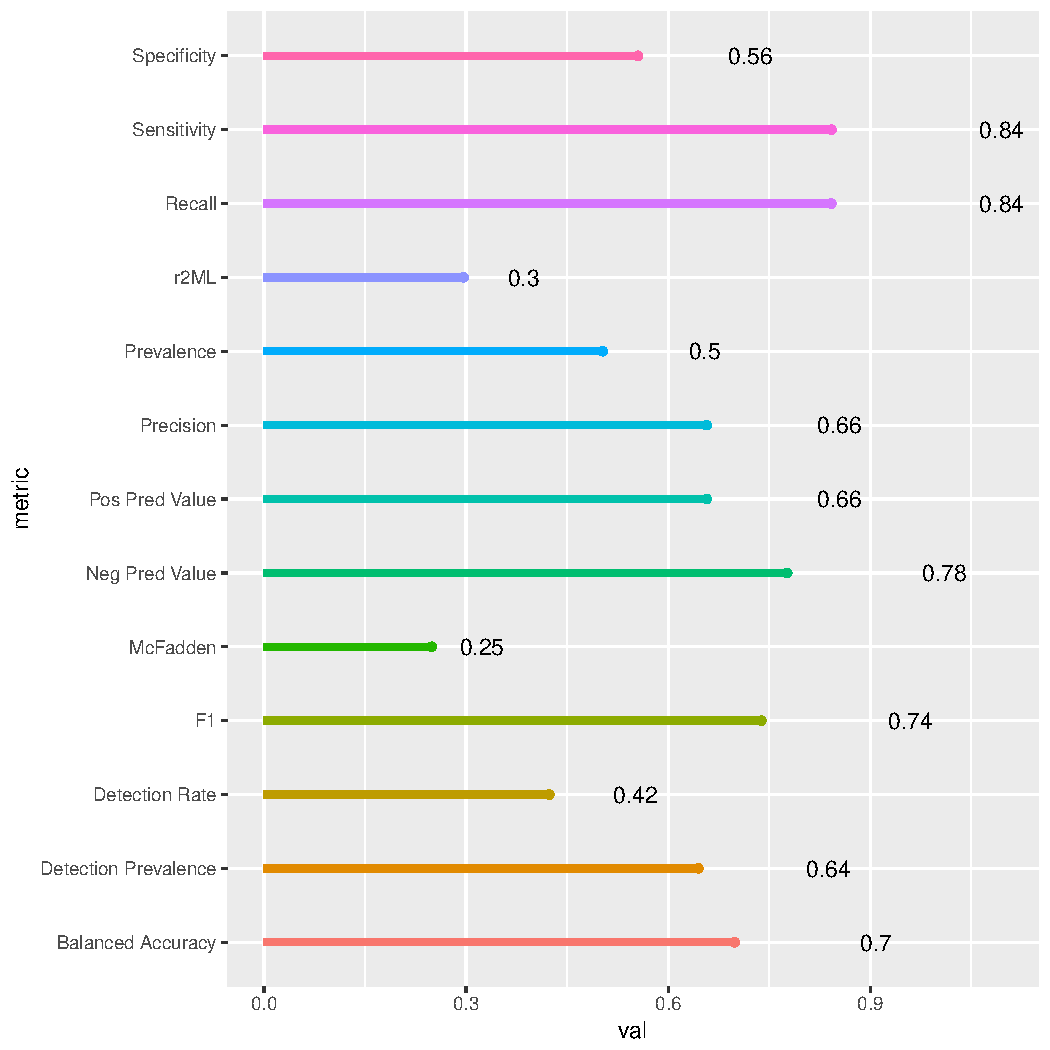
\includegraphics[width=0.8\textwidth]{/Users/charlvanschoor/Documents/Gottingen/ML/ML-Applications-CVS/LDA_consumer_analysis/src/output/confusion-metrics/conf-metrics-_NUM_TOPICS100.pdf}
\end{figure}




% subsection logistic_regression (end)
\subsection{Neural Network} % (fold)
\label{sub:neural_network}

Figures 9 to 12 show the results for the neural network. Each figure reports the results for the models with 10, 50 and a 100 topics. Figure 9 and 10 show the accuracy and loss values for the test dataset. As visible from Figure 9, the neural network has a higher level of accuracy than the logistic regression; around 79 percent for a 100 topics. 

\

Furthermore, the loss function in Figure 10 shows that there is a steady decrease in the loss from the model error, indicating that the model trained well\footnote{The model can be set to learn even slower with smaller batch sizes and more epochs, but this is left for future work.}. Figures 11 and 12 show the validation set accuracy and loss. The errors, or losses in Figure 12, are spread around a mean and can be considered homoscedastic, indicating that the model is not overfitting the data. Thus the neural network improved upon the linear model's predictive power. It is also clear that a model with a 100 topics out-predicts models with a smaller set of topics. This is likely due to the extra information given to the network. It also opens up the question of which amount of topics is optimal, however this is a question for future work.

\begin{figure}[!h]
\caption{Test Accuracy}\centering
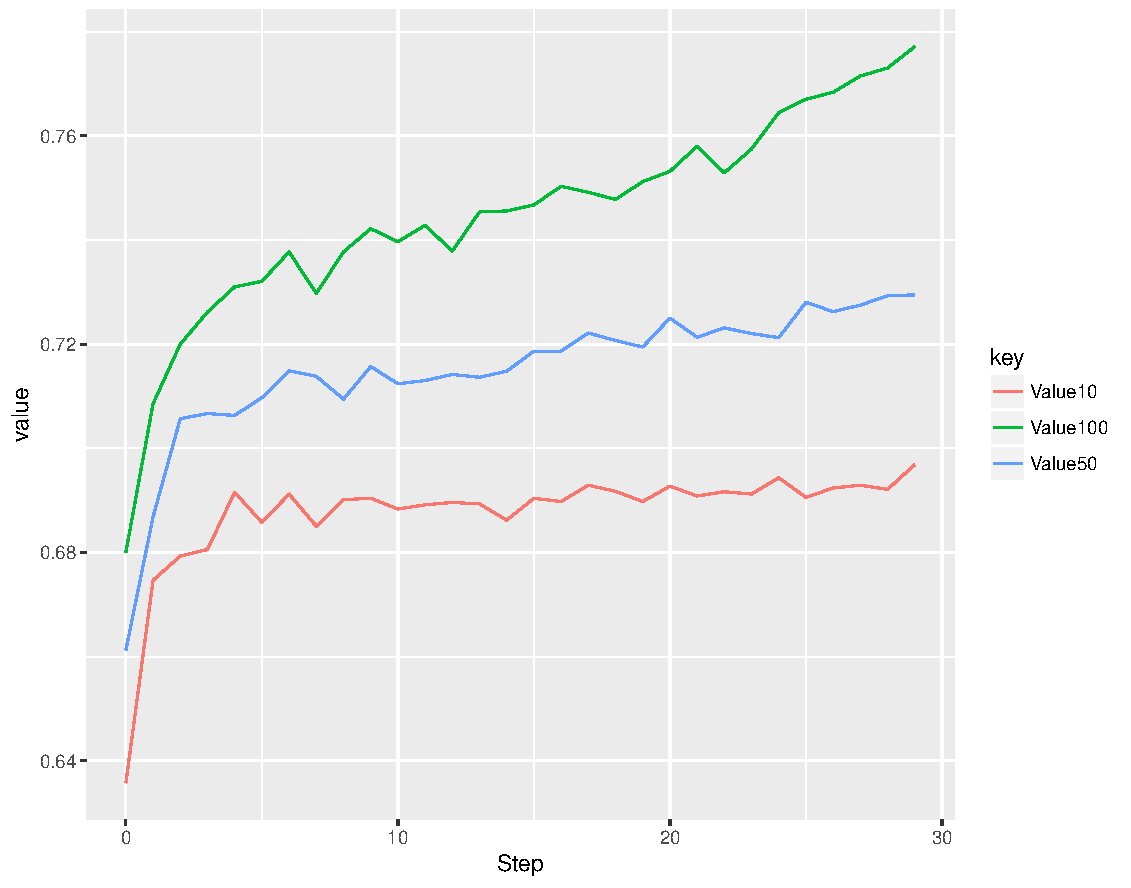
\includegraphics[width=0.7\textwidth]{/Users/charlvanschoor/Documents/Gottingen/ML/ML-Applications-CVS/LDA_consumer_analysis/src/runs/graphs/test_acc.pdf}
\end{figure}


\begin{figure}[!h]
\caption{Test Loss}\centering
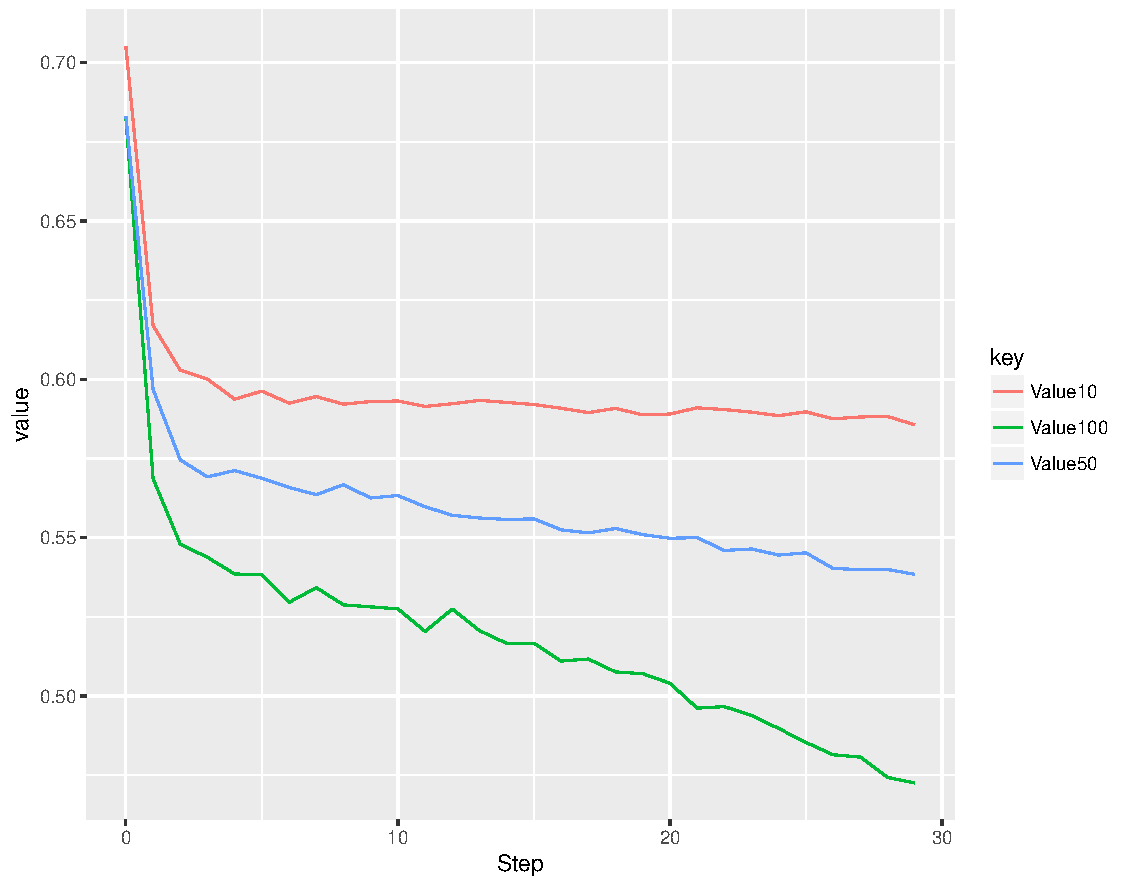
\includegraphics[width=0.7\textwidth]{/Users/charlvanschoor/Documents/Gottingen/ML/ML-Applications-CVS/LDA_consumer_analysis/src/runs/graphs/test_loss.pdf}
\end{figure}


\begin{figure}[!h]
\caption{Validation Accuracy}\centering
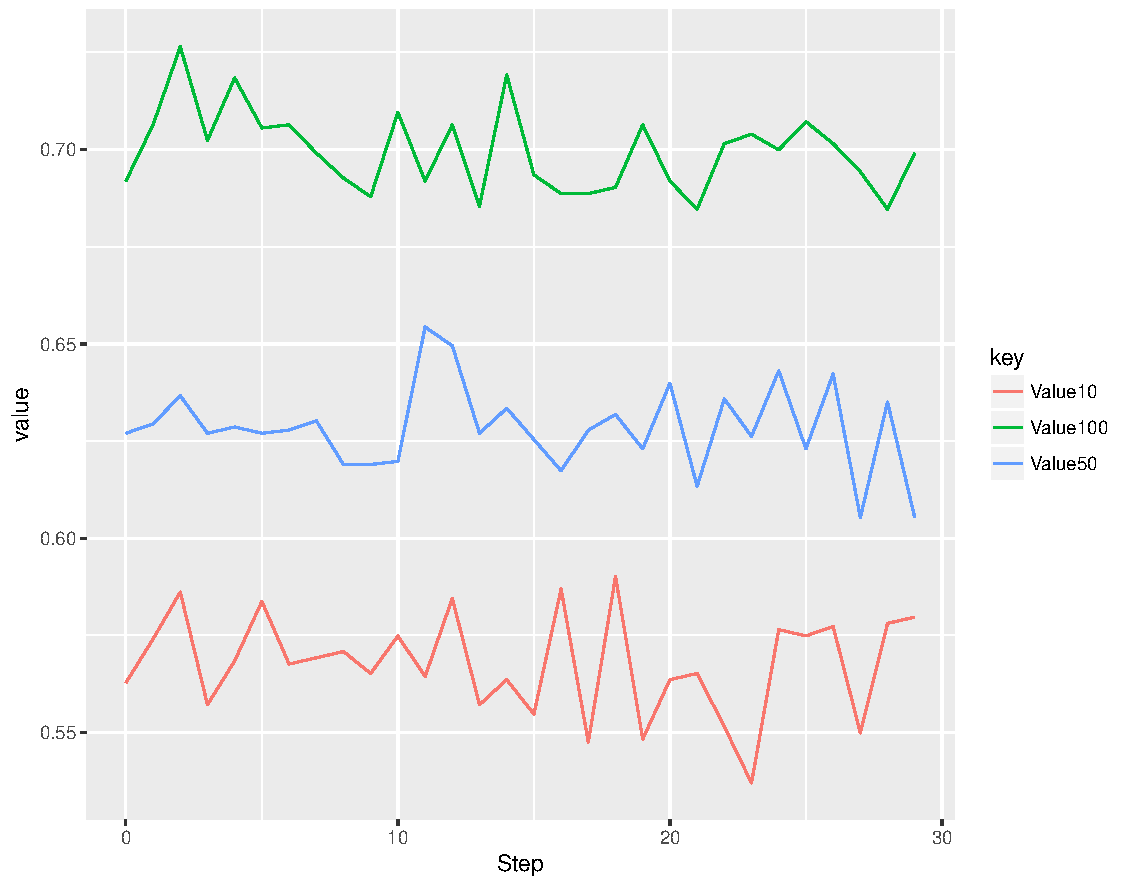
\includegraphics[width=0.7\textwidth]{/Users/charlvanschoor/Documents/Gottingen/ML/ML-Applications-CVS/LDA_consumer_analysis/src/runs/graphs/val_acc.pdf}
\end{figure}


\begin{figure}[!h]
\caption{Validation Loss}\centering
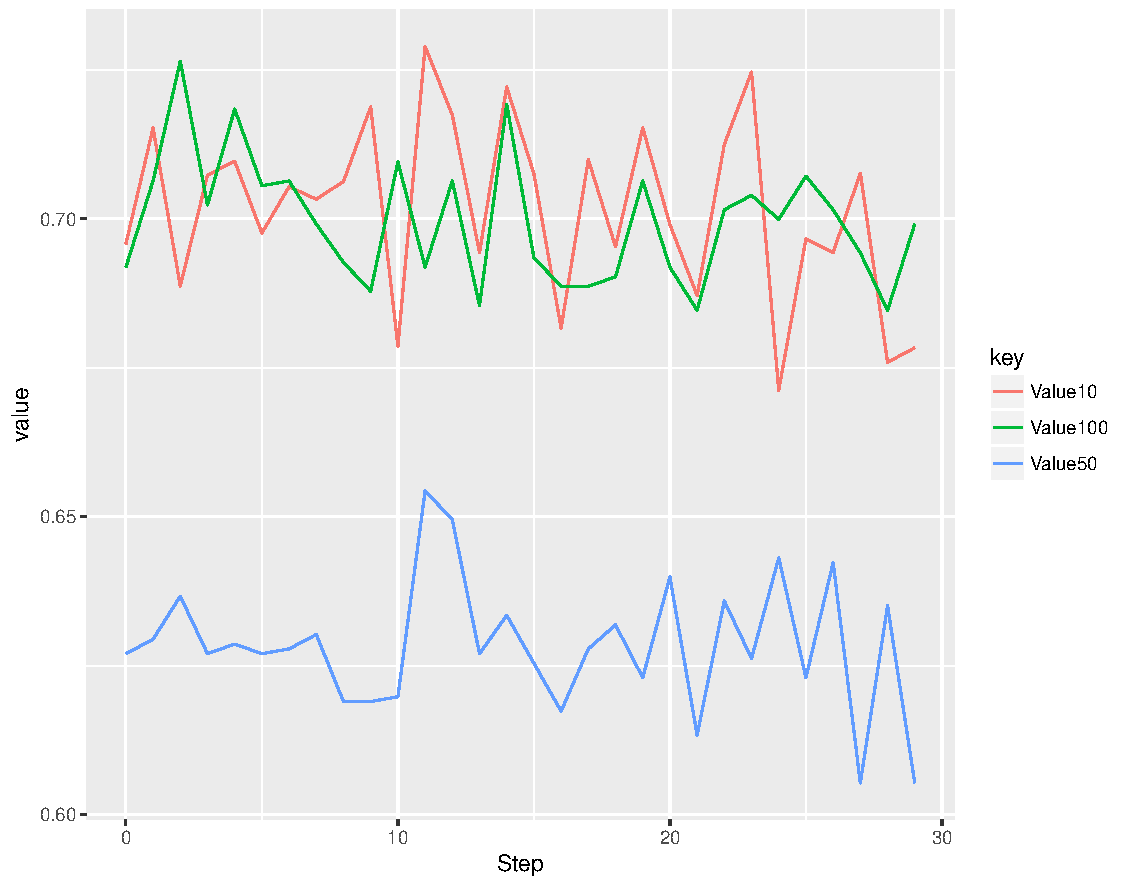
\includegraphics[width=0.7\textwidth]{/Users/charlvanschoor/Documents/Gottingen/ML/ML-Applications-CVS/LDA_consumer_analysis/src/runs/graphs/val_loss.pdf}
\end{figure}

% subsection neural_network (end)

% section results (end)